\chapter{Chapter 1: Introduction}\label{Chap:Introduction}
\textit{In vitro} techniques to model mammalian biology have long depended on the use of 2D cell culture in polystyrene dishes, while rat and mouse \textit{in vivo} models have been used to study whole organisms. These two tools, while at opposite ends of the spectrum of model complexity have provided us with much of what we know about human biology and have led to the development of countless therapies to treat a spectrum of human malignancies. Translating discoveries into useful medicine is incredibly difficult and new compounds entering FDA phase 1 clinical trials have a 10-15\% likelihood of approval \cite{Hay2014ClinicalDrugs}. Many of these compounds enter clinical trials after \textit{in vitro} or \textit{in vivo} models show initial success. The low success rates show that these models have inherent artifacts resulting in the failure to adequately reproduce appropriate human biological and physiological responses to many compounds and may call into question the relevance of these models to other biological phenomena they were used to study. Simple 2D models lack physiological context to be truly relevant, while many discoveries made in rodents do not transfer to humans due to differences in physiology. Issues with classical biological models have have not gone unnoticed and there have been great efforts to develop engineered \textit{in vitro} models that can replicate human tissues, organs, and even organ systems. The rationalization is that increased but controllable complexity will lead to increased relevance of the models and biological insights gained from studying them can be better applied to human medicine. I describe how engineered \textit{in vitro} models can be designed, fabricated, and used to investigate key components such as cell-cell, cell-matrix, and cell-drug interactions in the complex space of the tumor microenvironment (specifically multiple myeloma).  

\section{\textit{In vitro} tissue culture techniques}



\section{Microfluidics for Tissue culture}

\begin{figure}[ht] %DONE
\centering
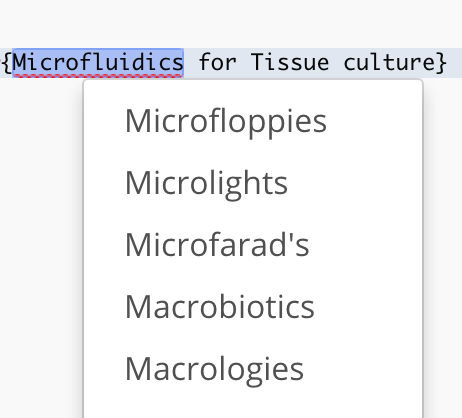
\includegraphics[width=4.5in]{/Test.png}
\caption{\textbf{The two-well hanging droplet device, operation, and capabilities}. (A) Two 8- device arrays of the two-well hanging droplet device with a close-up image and rendered-model of a single device. (B) Operation of a filled device containing cells, when fluid is removed or added through the interface well, volume of the culture well is changed with minimal disturbance to the culture. (C) Schematic of a dynamic coculutre experiment performed by combining two tissues in the hanging droplet device then separating the tissues.}
\label{figure:test}
\end{figure}



